\documentclass[times, utf8, zavrsni, numeric]{fer}
\usepackage{booktabs}
\usepackage[table]{xcolor}
\usepackage{amsmath}
\usepackage{graphicx}

\usepackage{listings}
\usepackage{color}
\usepackage{setspace}
%\definecolor{dkgreen}{rgb}{0,0.6,0}
\definecolor{gray}{rgb}{0.5,0.5,0.5}
%\definecolor{mauve}{rgb}{0.58,0,0.82}
\definecolor{black}{rgb}{0.0, 0.0, 0.0}

\renewcommand\lstlistingname{Ispis}
\renewcommand\lstlistlistingname{Popis ispisa}

\lstset{
mathescape,
frame=tb,
language=C,
aboveskip=3mm,
belowskip=3mm,
showstringspaces=false,
columns=flexible,
basicstyle={\small\ttfamily},
numbers=left,
numberstyle=\small\color{black},
keywordstyle=\color{black},
commentstyle=\color{black},
stringstyle=\color{black},
breaklines=true,
breakatwhitespace=true,
tabsize=2
}

\begin{document}

\thesisnumber{3253}

\title{GPU implementacija vremenski i memorijski učinkovitoga paralelnog algoritma za poravnanje slijedova}

\author{Marija Mikulić}

\maketitle

% Ispis stranice s napomenom o umetanju izvornika rada. Uklonite naredbu \izvornik ako želite izbaciti tu stranicu.
\izvornik

\zahvala{Hvala Mili što me motivirao da se posvetim računarstvu, na ukazanom povjerenju, na prenesenom znanju i ponajviše na strpljenju.}

\tableofcontents

\listoftables

\listoffigures

\chapter{Uvod}

\indent

Od svojih začetaka u 1940-ima, računala su postupno postala dio naše svakodnevice. To je područje ljudskog djelovanja koje se najbrže mijenja i evoluira. Ta evolucija se događa velikim dijelom zbog toga što se računala sve više i na sve više različitih načina primjenjuju u raznim područjima ljudskog djelovanja.

Jedno od tih područja je i biologija. U biologiji su za neke probleme, poput poravnavanja proteina i DNA, računala ključni alat za dolaženje do novih spoznaja. Iz te neodvojive veze nastalo je cijelo područje istraživanja koje nazivamo bioinformatika.

Biolozi ulažu velike napore u proučavanje našeg građevnog materijala, proteina i molekula DNA koji nas tvore. Proučavanje ovih molekula pokazalo se kao vrlo bitno i potencijalno vrlo korisno.

Primjerice, ako bismo mogli manipulirati svojom DNA, mogli bismo ukloniti iz svojih gena mnoge bolesti i sindrome koji danas, nažalost, pogađaju mnoge ljude.

Naravno, to otvara vrata i mnogim drugim stvarima te je predmet brojnih etičkih i filozofskih rasprava, ali prvotni cilj znanosti jest nastojati objasniti kako funkcionira svijet oko nas. Stoga nam je vrlo zanimljivo proučavati kako, u svojoj srži, funkcioniramo mi sami.

Iz te znatiželje i iz činjenice da su u biološkim molekulama spremljeni gigabajti informacija, pojavila se potreba za razvijanjem algoritama kojima bi se moglo učinkovito obrađivati tolike količine informacija.

Konkretan problem kojim se bavi ovaj završni rad jest poravnavanje jednog proteina s listom proteina. Odnosno, zanima nas koliko ima sličnosti između nekog proteina i \textit{N} drugih proteina. Ovaj rad opisuje rješenje toga problema algoritmom koji koristi predmetačni račun i Smith-Watermanov algoritam.

Poglavlje 2 opisuje općenito problem poravnavanja struktura. U poglavlju 3 izložen je Smith-Watermanov algoritam, a u poglavlju 4 predmetačni račun.
Poglavlje 5 opisuje tehnologiju CUDA, a poglavlje 6 specifičnosti implementacije, dok se u poglavlju 7 izlažu dobiveni rezultati. Poglavlje 8 posvećeno je zaključku rada.


\chapter{Poravnavanje struktura}
\indent

Kao jedan od ključnih problema bioinformatike nametnuo se problem poravnanja molekula proteina i DNA. Svrha tog poravnanja jest ustanoviti područja sličnosti između tih struktura, jer ona mogu indicirati funkcijsku, strukturalnu ili evolucijsku vezu između njih\cite{salign}.

Za potrebe informatike, problem poravnanja struktura se može svesti na problem poravnavanja slijedova znakova. Za ilustraciju, zamislimo da se slijedovi koje poravnavamo stave jedan ispod drugog. U tom slučaju, cilj je tako postaviti znakove nizova da oni izgledaju najsličnije moguće.

Razlikujemo dvije vrste poravnavanja: globalno i lokalno.

Globalno poravnavanje je postupak kojim se jedan slijed preslikava na drugi od početka do kraja. Pri tome je dozvoljeno u bilo koji slijed umetnuti prazninu na proizvoljno mjesto, osim na prvo. Ukoliko je jedan slijed znatno dulji od drugog, ovakvo poravnanje može za posljedicu imati umetanje velikog broja praznina u kraći slijed.

Za razliku od globalnog, lokalno poravnanje ne vodi računa o tome da se iskoriste svi znakovi oba slijeda. Ovdje je cilj naći podslijedove zadanih slijedova koji su međusobno najsličniji. S obzirom na to da se ne moraju iskoristiti svi znakovi bilo kojeg slijeda, nije dozvoljeno da optimalno poravnanje počinje ili završava prazninom.

\begin{figure}[ht!]
\centering
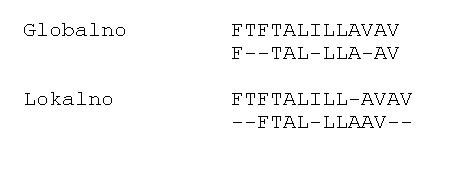
\includegraphics[width=90mm]{poravnanje.png}
\caption{Primjer globalnog i lokalnog poravnanja dvaju nizova}
\label{poravnanje}
\end{figure}

\chapter{Smith-Watermanov algoritam}
\indent

Smith-Watermanov algoritam\cite{swarticle} među najvažnijim je algoritmima za lokalno poravnanje slijedova. Budući da je algoritam nastao iz Needleman-Wunschovog\cite{nwarticle} algoritma za globalno poravnanje slijedova, prvo ćemo razmotriti taj algoritam pa predstaviti potrebne modifikacije kako bismo dobili Smith-Watermanov algoritam za lokalno poravnanje slijedova.

\section{Needleman-Wunschov algoritam}
\indent

Poznat još i kao algoritam optimalnog poravnanja, Needleman-Wunschov algoritam koristi se za globalno poravnavanje slijedova. To je prvi algoritam koji je primijenio dinamičko programiranje na problem poravnanja slijedova u biologiji.

\subsection{Algoritam}
\indent 

Cilj Needleman-Wunschovog algoritma jest pronaći optimalno poravnanje neka dva slijeda A i B, odnosno ono poravnanje koje u obzir uzima sve znakove oba slijeda i usto ima najviši broj bodova s obzirom na sva moguća poravnanja (dozvoljeno je postojanje više rješenja s istim brojem bodova).

Označimo s $n$ duljinu slijeda A i s $m$ duljinu slijeda B. Za potrebe pronalaska optimalnog globalnog rješenja potrebno je alocirati dvodimenzionalnu matricu dimenzija $(n + 1) \times (m + 1)$. Nulti redak i stupac služe za inicijalizaciju matrice. Gledajući od indeksa 1, svaki redak matrice predstavlja znak u slijedu A, a svaki stupac predstavlja znak u slijedu B. Element matrice $F_{ij}$, gdje je $i$ indeks retka, a $j$ indeks stupca, predstavlja broj bodova za poravnanje prvih $i$ znakova slijeda A i prvih $j$ znakova slijeda B.

Kako bismo ocijenili poravnanje neka dva znaka, definiramo \textit{matricu sličnosti} \textbf{S} nad skupom dozvoljenih znakova $\Sigma$. Element matrice $S_{\sigma_{i}, \sigma_{j}}$ daje ocjenu poravnanja znaka $\sigma_{i}$ sa znakom $\sigma_{j}$. Dodatno, potrebno je ocijeniti umetanje praznina u bilo koji od dva slijeda. Za te potrebe definira se konstanta $d$ $(d < 0)$ kojom se kažnjava svaka praznina.

Pošto tražimo optimalno globalno poravnanje, želimo biti sigurni da će poravnanje krenuti od prvog znaka slijeda A i prvog znaka slijeda B. Zbog toga se postavljaju sljedeći početni uvjeti:
\begin{center}
$F_{0j} = d \times j,\hspace{50pt} j = 0...m - 1$\\
$F_{i0} = d \times i,\hspace{50pt} i = 0...n - 1$
\end{center}
Svi ostali elementi matrice računaju se prema formuli:
\begin{center}
\begin{equation}
F_{i, j} = \max \left\{
	\begin{array}{lr}
		F_{i-1,j-1} + S(A_{i}, B_{j}) \\
		F_{i, j-1} + d \\
		F_{i-1, j} + d
	\end{array}
\right.
\end{equation}
\end{center}

Nakon što su izračunati svi elementi matrice, element $F_{nm}$ sadrži broj bodova optimalnog globalnog poravnanja.

\subsection{Primjer}
\indent

Za ilustraciju rada algoritma poslužit će primjer poravnanja DNA slijedova \emph{AGACTAGTTAC} i \emph{CGAGACGT}.

Nad abecedom (koja je u ovom slučaju \{A, C, G, T\}) definira se sljedeća matrica sličnosti \textbf{S}:
\begin{table}[hb]
\begin{center}
\begin{tabular}{r | r r r r}
 & \textbf{A} & \textbf{G} & \textbf{C} & \textbf{T} \\
\hline
\textbf{A} & 10 & -1 & -3 & -4\\
\textbf{G} & -1 & 7 & -5 & -3\\
\textbf{C} & -3 & -5 & 9 & 0\\
\textbf{T} & -4 & -3 & 0 & 8\\
\end{tabular}
\end{center}
\caption{Primjer matrice sličnosti}
\label{table:matricaslicnosti}
\end{table}
Usto, neka je vrijednost funkcije kazne $d = -5$. Nakon izvođenja algoritma, matrica \textbf{F} sadrži sljedeće vrijednosti:
\begin{table}[h]
\begin{center}
\begin{tabular}{| r | r r r r r r r r r r r r |}
\hline
 &  & A & G & A & C & T & A & G & T & T & A & C \\
\hline
 & \cellcolor{lightgray}0 & -5 & -10 & -15 & -20 & -25 & -30 & -35 & -40 & -45 & -50 & -55\\
C & -5 & \cellcolor{lightgray}-3 & -8 & -13 & -6 & -11 & -16 & -21 & -26 & -31 & -36 & -41\\
G & -10 & -6 & \cellcolor{lightgray}4 & -1 & -6 & -9 & -12 & -9 & -14 & -19 & -24 & -29\\
A & -15 & 0 & -1 & \cellcolor{lightgray}14 & 9 & 4 & 1 & -4 & -9 & -14 & -9 & -14\\
G & -20 & -5 & 7 & \cellcolor{lightgray}9 & 9 & 6 & 3 & 8 & 3 & -2 & -7 & -12\\
A & -25 & -10 & 2 & \cellcolor{lightgray}17 & 12 & 7 & 16 & 11 & 6 & 1 & 8 & 3 \\
C & -30 & -15 & -3 & 12 & \cellcolor{lightgray}26 & 21 & 16 & 11 & 11 & 6 & 3 & 17 \\
G & -35 & -20 & -8 & 7 & 21 & \cellcolor{lightgray}23 & \cellcolor{lightgray}20 & \cellcolor{lightgray}23 & 18 & 13 & 8 & 12 \\
T & -40 & -25 & -13 & 2 & 16 & 29 & 24 & 19 & \cellcolor{lightgray}31 & \cellcolor{lightgray}26 & \cellcolor{lightgray}21 & \cellcolor{lightgray}16 \\
\hline
\end{tabular}
\end{center}
\caption{Matrica \textbf{F} nakon provedbe Needleman-Wunschovog algoritma}
\label{table:nwmatrica}
\end{table}

Vidimo da optimalno poravnanje ima broj bodova 16 i da su slijedovi poravnati na sljedeći način:

\begin{table}[h]
\begin{center}
\begin{tabular}{r r r r r r r r r r r r r}
A & G & A & - & - & C & T & A & G & T & T & A & C \\
C & G & A & G & A & C & G & - & - & T & - & - & - \\
\end{tabular}
\end{center}
\caption{Globalno poravnati slijedovi}
\label{table:nwporavnanje}
\end{table}

\section{Smith-Watermanov algoritam}
\indent

Za razliku od Needleman-Wunschovog, Smith-Watermanov algoritam koristi se za lokalno poravnanje slijedova. Ideja algoritma je ista, ali su potrebne modifikacije.

Ostat ćemo pri istim oznakama: razmatramo slijedove A (duljine $n$) i B (duljine $m$) definirane nad abecedom $\Sigma$. S $d$ ćemo označavati kaznene bodove za umetanje praznine, a poravnanje neka dva elementa abecede $\Sigma$ definirano je matricom sličnosti \textbf{S}. Potrebno je popuniti matricu \textbf{F}.

Pošto poravnanje ne mora početi s prvim znakovima oba niza, kao donja granica poravnanja postavi se vrijednost 0. Ovo omogućuje da poravnanje prekinemo kad postane nepovoljno, odnosno kad bi ocjena poravnanja postala negativna, i krenemo razmatrati poravnanje koje počinje nekim drugim znakom. S obzirom na ovaj zahtjev, početni uvjeti su sljedeći:
\begin{center}
$F_{0j} = 0,\hspace{50pt} j = 0...m - 1$\\
$F_{i0} = 0,\hspace{50pt} i = 0...n - 1$
\end{center}
a algoritam je modificiran tako da ne dopušta negativno poravnanje:
\begin{center}
\begin{equation}
F_{i,j} = \max \left\{
	\begin{array}{lr}
		F_{i-1,j-1} + S(A_{i}, B_{j}) \\
		F_{i, j-1} + d \\
		F_{i-1, j} + d \\
		0
	\end{array}
\right.
\end{equation}
\end{center}

\begin{table}[hbt]
\begin{center}
\begin{tabular}{| r | r r r r r r r r r r r r |}
\hline
 &  & A & G & A & C & T & A & G & T & T & A & C \\
\hline
  & 0 & 0 & 0 & 0 & 0 & 0 & 0 & 0 & 0 & 0 & 0 & 0 \\
C & 0 & 0 & 0 & 0 & 9 & 4 & 0 & 0 & 0 & 0 & 0 & 9 \\
G & 0 & 0 & 7 & 2 & 4 & 6 & 3 & 7 & 2 & 0 & 0 & 4 \\
A & 0 & \cellcolor{lightgray}10 & 5 & 17 & 12 & 7 & 16 & 11 & 6 & 1 & 10 & 5 \\
G & 0 & 5 & \cellcolor{lightgray}17 & 12 & 12 & 9 & 11 & 23 & 18 & 13 & 8 & 5 \\
A & 0 & 10 & 12 & \cellcolor{lightgray}27 & 22 & 17 & 19 & 18 & 19 & 14 & 23 & 18 \\
C & 0 & 5 & 7 & 22 & \cellcolor{lightgray}36 & \cellcolor{lightgray}31 & 26 & 21 & 18 & 19 & 18 & 32 \\
G & 0 & 0 & 12 & 17 & 31 & \cellcolor{lightgray}33 & \cellcolor{lightgray}30 & \cellcolor{lightgray}33 & 28 & 23 & 18 & 27 \\
T & 0 & 0 & 7 & 12 & 26 & 39 & 34 & 29 & \cellcolor{lightgray}41 & 36 & 31 & 26 \\
\hline
\end{tabular}
\end{center}
\caption{Matrica \textbf{F} nakon provedbe Smith-Watermanovog algoritma}
\label{table:swmatrica}
\end{table}

\begin{table}[hbt]
\begin{center}
\begin{tabular}{c c c c c c c c c c c c c c}
 & & A & G & A & C & T & - & A & G & T & \color{lightgray}T & \color{lightgray}A & \color{lightgray}C\\
\color{lightgray}C & \color{lightgray}G & A & G & A & C & - & G & - & - & T & & & \\
\end{tabular}
\end{center}
\caption{Najbolje lokalno poravnanje}
\label{table:swporavnanje}
\end{table}

\subsection{Kažnjavanje praznina}
\indent

Opisani algoritam kao funkciju kazne koristi \emph{linearnu} funkciju kazne - svaka praznina se kažnjava s $d$ bodova, što znači da je praznina duljine $k$ ocijenjena s $k\cdot d$. Međutim, kako bi bio kvalitetan za poravnanje bioloških struktura (proteina i nizova DNA), ovaj algoritam potrebno je dodatno modificirati.

Naime, praznine koje se umeću u slijedove predstavljaju mutacije, a veća je vjerojatnost da se dogodila jedna mutacija nad nekim podslijedom nego nekoliko mutacija nad jednim elementom niza zaredom.

Empirijski dokazana formula za ocjenjivanje procjepa jest parabola. Stoga se definira afina funkcija kazne, koja za produljenje postojeće praznine dodjeljuje manju kaznu nego za otvaranje nove. Označimo s $o$ $(o < 0)$ kaznu za otvaranje praznine i s $e$ $(o < e < 0)$ kaznu za produljenje postojeće praznine. Tada je za prazninu duljine $n$ kazna  $o + (n - 1)e$. Uporabom ovakve funkcije dobiju se najbolji praktični rezultati.\cite{gapopen}

S obzirom na ovu promjenu, potrebno je modificirati i sam algoritam, što nije trivijalno. Označimo s A slijed koji ćemo postaviti kao referentni za retke matrice, a s B slijed koji je referentan za stupce matrice \textbf{F}.

Kako bismo uspješno pratili sve moguće situacije, potrebne su nam tri matrice: \textbf{N} (\emph{no gaps - bez procjepa}), koja pokušava poravnati iduća dva elementa slijedova, \textbf{H} (\emph{horizontal gap - umetanje}), koja pokušava idući element slijeda B poravnati s prazninom i \textbf{V}(\emph{vertical gap - brisanje}), koja pokušava idući element slijeda A poravnati s prazninom.

Početni uvjeti za sve tri matrice su:
\begin{center}
$N_{0j} = 0, H_{0j} = 0, V_{0j} = 0,\hspace{50pt} j = 0...m-1$\\
$N_{i0} = 0, H_{i0} = 0, V_{i0} = 0,\hspace{50pt} i = 0...n-1$
\end{center}

a ostali elementi matrica računaju se prema sljedećim formulama:
\begin{center}
\begin{equation}
H_{i,j} = \max \left\{
	\begin{array}{lr}
		N_{i,j-1} + o \\
		H_{i, j-1} + e \\
		0\\
	\end{array}
\right.
\end{equation}
\begin{equation}
V_{i,j} = \max \left\{
	\begin{array}{lr}
		N_{i-1,j} + o \\
		V_{i-1, j} + e \\
		0\\
	\end{array}
\right.
\end{equation}
\begin{equation}
N_{i,j} = \max \left\{
	\begin{array}{lr}
		N_{i-1,j-1} + S(A_{i}, B_{j}) \\
		H_{i, j}\\
		V_{i, j}\\
		0\\
	\end{array}
\right.
\end{equation}
\end{center}

\chapter{Predmetačni račun}
\indent

Problem predmetačnog računa definira se pomoću niza A = \{a$_{0}$, a$_{1}$, a$_{2}$, ..., a$_{n-1}$\} i općenitog binarnog operatora $\oplus$. Cilj nam je generirati niz B. 

Postoje dvije vrste predmetačnog računa: uključivi i isključivi.
Kako bismo proveli uključivi predmetačni račun, svaki element $b_{i}$ niza B izračuna se tako da se primijeni operator $\oplus$ na sve elemente niza A od $a_{0}$ do $a_{i}$ ($i = 0...n-1$).
Za razliku od uključivog, isključivi predmetačni račun za izračun elementa $b_{i}$ ne koristi element $a_{i}$. Odnosno, element $b_{i}$ niza B izračuna se tako da se na sve elemente niza A od $a_{0}$ do $a_{i - 1}$ ($i = 0...n-1$) primijeni operator $\oplus$. Ovakvim postupkom ostaje nepoznat element $b_{0}$. Na to mjesto doda se element koji je neutralan s obzirom na operator $\oplus$.

Dakle, ovisno o vrsti predmetačnog računa koju želimo upotrijebiti, niz B može sastoji se od sljedećih elemenata:
\begin{itemize}
\item B = \{$0, 0 \oplus a_{0}, 0 \oplus a_{0} \oplus a_{1}, ..., 0 \oplus a_{0} \oplus ... \oplus a_{n-2}$\}
\item B = \{$a_{0}, a_{0} \oplus a_{1}, a_{0} \oplus a_{1} \oplus a_{2}, ..., a_{0} \oplus a_{1} \oplus ... \oplus a_{n-1}$\}
\end{itemize}

Ovaj se problem pojavljuje često kao usko grlo u raznovrsnim problemima. Neki od njih su:
\begin{itemize}
\item leksička usporedba nizova znakova (npr. određivanje da niz "strategija" dolazi ispred niza "strateški" u rječniku)
\item paralelno ostvarenje \textit{radix-sort} i \textit{quick-sort} algoritama
\item određivanje vidljivosti točaka u 3D krajoliku – uz operator \textit{max}
\item zbrajanje s brojevima višestruke (proizvoljne) preciznosti
\item alokacija procesora/memorije
\item pretraživanje regularnih izraza (npr. u implementaciji \textit{grep} naredbe u \textit{UNIX}-u)
\item izvedba nekih operacija nad stablima (npr. dubina svakog čvora u stablu)
\end{itemize}

\section{Primjer}

Za ilustraciju problema, razmotrimo slijedeći primjer:
Zadan je niz A:
\begin{center}
\begin{tabular}{| r | r | r | r | r | r | r | r | r |}
\hline
\cellcolor{lightgray}indeks & \cellcolor{lightgray}0 & \cellcolor{lightgray}1 & \cellcolor{lightgray}2 & \cellcolor{lightgray}3 & \cellcolor{lightgray}4 & \cellcolor{lightgray}5 & \cellcolor{lightgray}6 & \cellcolor{lightgray}7 \\
\hline
vrijednost & 5 & 3 & -8 & 4 & 12 & 6 & -9 & 1\\
\hline
\end{tabular}
\end{center}

Ako je binarni operator "+" i izvodimo uključivi predmetačni račun, tada je cilj dobiti sljedeći niz B:
\begin{center}
\begin{tabular}{| r | r | r | r | r | r | r | r | r |}
\hline
indeks & 0 & 1 & 2 & 3 & 4 & 5 & 6 & 7\\
\hline
vrijednost & 5 & 8 & 0 & 4 & 16 & 22 & 13 & 14\\
\hline
\end{tabular}
\end{center}
Ako pak za isti primjer izvedimo isključivi predmetačni račun, niz B izgleda ovako:
\begin{center}
\begin{tabular}{| r | r | r | r | r | r | r | r | r |}
\hline
\cellcolor{lightgray}indeks & \cellcolor{lightgray}0 & \cellcolor{lightgray}1 & \cellcolor{lightgray}2 & \cellcolor{lightgray}3 & \cellcolor{lightgray}4 & \cellcolor{lightgray}5 & \cellcolor{lightgray}6 & \cellcolor{lightgray}7 \\
\hline
vrijednost & 0 & 5 & 8 & 0 & 4 & 16 & 22 & 13\\
\hline
\end{tabular}
\end{center}

Očito je da se isključivi predmetačni račun jednostavno generira iz uključivog tako da se svi elementi pomaknu za jedno mjesto udesno, a kao nulti element se doda neutralni element.


\section{Algoritam}

\indent

Predmetačni račun je jedan od algoritama koji se čine inherentno sekvencijalnima, ali za koje postoji učinkovita paralelna implementacija. Budući da se u ovom radu koristi isključivi predmetačni račun, razmotrit ćemo algoritam nad njime.

\subsection{Sekvencijalni algoritam}

\indent

Sekvencijalna implementacija ovog algoritma je trivijalna i svodi se na dinamičko programiranje. Verzija algoritma sa binarnim operatorom "+" (predmetačni zbroj) dana je u ispisu:

\begin{figure}[hbt]
\begin{singlespace}
\begin{lstlisting}[label={predmetacni zbroj}]
b[0] := 0
za svaki k od 1 do n-1
	b[k] := a[k-1] + b[k-1]
\end{lstlisting}
\end{singlespace}
\caption{Algoritam za predmetačni zbroj}
\label{prefixsumalgoritam}
\end{figure}

\subsection{Paralelni algoritam}
\indent

Učinkovita paralelna implementacija predmetačnog računa temelji se na radu Blellocha \cite{blelloch} i koristi balansirano stablo. Ideja je izgraditi balansirano binarno stablo nad ulaznim podacima i zatim njegovim obilaskom do listova do korijena pa od korijena do listova napraviti račun.

Binarno stablo s $n$ listova ima dubinu $d = log_{2}n$, a svaka dubina ima $2^{d}$ čvorova. Ako izvodimo jedan izračun po čvoru, u jednom obilasku stabla izvodimo $O(n)$ izračuna. Ovo binarno stablo nije fizički implementirano, nego je koncept koji koristimo kako bismo odredili što je zadatak svake dretve u obilasku stabla, a svi izračuni izvode se nad ulaznim nizom podataka.

Izračun se izvodi u dvije faze: reduciranje i predtraženje.

U fazi reduciranja, stablo se obilazi od listova do korijena i izvode se djelomični izračuni, te na kraju ove faze korijen stabla sadrži izračun za sve čvorove u stablu.

Slika i ispis predstavljaju fazu reduciranja na gore navedenom primjeru.

\begin{figure}[ht!]
\centering
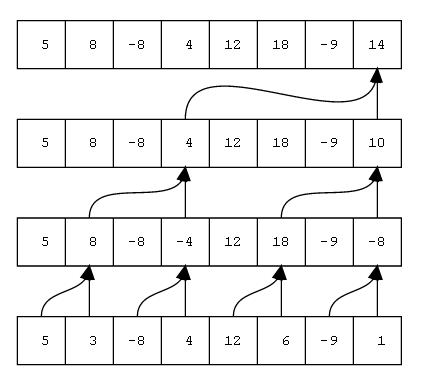
\includegraphics[width=90mm]{redukcija.png}
\caption{Faza redukcije}
\label{redukcija}
\end{figure}

\begin{figure}[hbt]
\begin{singlespace}
\begin{lstlisting}[label={reduciranje}]
za svaki d od 0 do log$_{2}$n - 1:
	za svaki k od 0 do n - 1 s korakom 2$^{d+1}$ u paraleli:
		a[k + 2$^{d+1}$ - 1] = a[k + 2$^{d}$ - 1] + a[k + 2$^{d+1}$ - 1]
\end{lstlisting}
\end{singlespace}
\caption{Algoritam faze redukcije}
\label{redukcijaalgoritam}
\end{figure}

U fazi predtraženja stablo se obilazi od korijena do listova i koriste se djelomični izračuni iz faze reduciranja kako bismo izveli predmetačni račun za svaki element.

U korijen stabla se umetne neutralni element. Zatim, u svakom koraku čvor trenutne razine svom lijevom djetetu preda svoju vrijednost, a zbroj svoje vrijednosti i prethodne vrijednosti lijevog djeteta preda desnom djetetu.

Slika i ispis predstavljaju fazu predtraženja na gore navedenom primjeru.
\pagebreak

\begin{figure}[Htb]
\centering
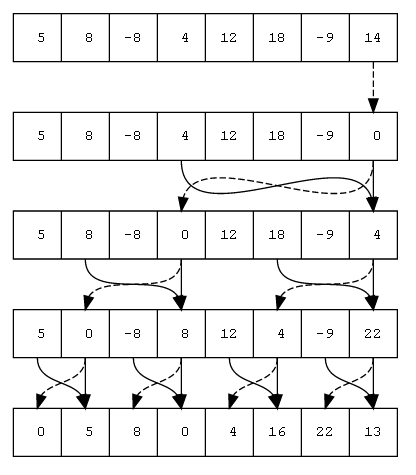
\includegraphics[width=90mm]{predtrazenje.png}
\caption{Faza predtraženja}
\label{predtrazenje}
\end{figure}

\begin{figure}[hbt]
\begin{singlespace}
\begin{lstlisting}[label={prescan}]
a[n-1] = 0
za svaki d od log$_{2}$n - 1 do 0:
	za svaki k od 0 do n - 1 s korakom 2$^{d}$ + 1:
		temp = a[k + 2$^{d}$ - 1]
		a[k + 2$^{d}$ - 1] = a[k + 2$^{d+1}$ - 1]
		a[k + 2$^{d+1}$ - 1] = temp + a[k + 2$^{d+1}$ - 1]
\end{lstlisting}
\end{singlespace}
\caption{Algoritam za fazu predtraženja}
\label{prescanalgoritam}
\end{figure}

\chapter{CUDA tehnologija}
\indent

Grafičke kartice su prvotno dizajnirane kao grafički ubrzivači i podržavale su cjevovode točno određenih funkcija. No, u 1990-im godinama doživjele su dramatičan razvoj i postajale sve više programabilne. NVIDIA, tvrtka koja je i skovala termin GPU (\emph{graphics processing unit} - \emph{grafička procesna jedinica}), svoj je prvi GPU proizvela 1999. Od tad su moć te tehnologije, osim proizvođača računalnih igara i umjetnika, prepoznali i mnogi istraživači te ju počeli koristiti za svoje potrebe.

Međutim, u to doba je bilo potrebno "prevariti" grafičku karticu koju se htjelo iskoristiti, to jest, trebalo podatke pretočiti u probleme koji se mogu prikazati trokutima i poligonima. Kako bi se to izbjeglo, razvio se GPGPU (\textit{general purpose graphics processing unit} - \textit{grafička procesna jedinica opće namjene}).

Uskoro su se pojavile i prilagodbe općih programskih jezika za novonastalu tehnologiju.

\textit{CUDA} tehnologija (punog naziva \textit{Compute Unified Device Architecture} - \textit{računski ujedinjena arhitektura uređaja}) je programski model i platforma za paralelno programiranje koju je razvila tvrtka NVIDIA i implementirala na svojim grafičkim procesnim jedinicama.\cite{cuda}

Prva verzija CUDA-inog SDK-a (engl. \textit{software development kit} - oprema za razvoj programske podrške) izdana je 15. veljače 2007. Ona je omogućila korištenje resursa grafičkih kartica jedino u programskom jeziku C. Od tada do danas izdane su još dvije velike iteracije i nekoliko manjih te danas možemo koristiti i podskup jezika C++ \cite{rahlezavrsni}.

Za shvaćanje načina rada grafičke procesne jedinice s \emph{CUDA} arhitekturom, moramo razumjeti sljedeće pojmove\cite{rahlezavrsni}:
\begin{itemize}
\item \emph{host} tj. domaćin - centralna procesna jedinica računala (\emph{CPU})
\item \emph{device} tj. uređaj - grafička procesna jedinica
\item \emph{thread} tj. dretva - najmanja jedinica izvršavanja, sve naredbe unutar dretve izvršavaju se slijedno
\item \emph{block} tj. blok - skup dretvi koje se izvršavaju paralelno
\item \emph{grid} tj. mreža - skup blokova koji se izvršavaju paralelno
\item \emph{warp} tj. osnova - skup dretvi unutar bloka koje se izvršavaju istodobno i za koje je dozvoljeno pretpostaviti da se u svakom trenutku nalaze na istom mjestu u kodu (stoga ih nije potrebno ručno sinkronizirati)
\end{itemize}

\chapter{Implementacija}
\indent

Ovaj rad modifikacija je rada Alurua i suradnika\cite{aluru}. Oni su pokazali kako se predmetačni račun može koristiti za ubrzanje postupka poravnanja dvaju bioloških slijedova. U svome radu opisuju postupak za globalno poravnanje slijedova.

Inovativnost ovog rada jest u tome da se jedan protein poravnava s $N$ proteina. Označimo protein koji poravnavamo s A, a listu proteina na koji poravnavamo protein A s L. Cilj je naći optimalno lokalno poravnanje između A i bilo kojeg proteina L[i] ($i = 0...N-1$).

Svi elementi L[i] ($i = 0...N-1$) konkatenirani su u jedan niz (nazovimo i njega L) i međusobno odvojeni znakom za prekid. Znak za prekid se koristi kako bismo mogli prekinuti pratiti trenutno poravnanje i krenuti s novim.

Kako bi se ocijenilo poravnanje neka dva elementa \emph{a} i \emph{l} abecede nad kojom su definirani slijedovi (označimo ju sa $\Sigma$), uvodi se jednostavna funkcija:
\begin{equation}
f(a, l) = \max \left\{
	\begin{array}{lr}
		1\hspace{50pt}a = l,\hspace{10pt}a,l \in \Sigma \\
		0\hspace{50pt}a \ne l,\hspace{10pt}a, l \in \Sigma
	\end{array}
\right.
\end{equation}
Kao funkcija kažnjavanja procjepa uvodi se afina funkcija kojom se otvaranje procjepa kažnjava s $o$, a produljenje postojećeg procjepa s $e$.

Kao što je prethodno opisano, koriste se tri matrice: \textbf{N}, \textbf{H} i \textbf{V}. Svaka matrica je dimenzija $(n + 1) \times (m + 1)$, gdje je $n$ duljina niza A, a $m$ duljina niza L. Početni uvjeti u matricama postavljaju se na sljedeći način:
\begin{center}
$N_{0j} = 0, H_{0j} = 0, V_{0j} = 0,\hspace{50pt} j = 0...m$\\
$N_{i0} = 0, H_{i0} = 0, V_{i0} = 0,\hspace{50pt} i = 0...n$\\
\end{center}
a preostali elementi matrica ($i = 1...n, j = 1...m$) pomoću formula:
\begin{center}
\begin{equation}
N_{i, j} = f(a_{i}, l_{j}) + \max
\left\{
	\begin{array}{lr}
	N_{i - 1, j - 1} \\	
	H_{i - 1, j - 1} \\
	V_{i - 1, j - 1} \\
	0\\
	\end{array}
\right.
\end{equation}
\begin{equation}
H_{i, j} = \max \left\{
	\begin{array}{lr}
	N_{i, j - 1} + o\\	
	H_{i, j - 1} + e\\
	V_{i, j - 1} + o\\
	0\\
	\end{array}
\right.
\end{equation}
\begin{equation}
V_{i, j} = \max \left\{
	\begin{array}{lr}
	N_{i - 1, j} + o \\	
	H_{i - 1, j} + o\\
	V_{i - 1, j} + e \\
	0\\
	\end{array}
\right.
\end{equation}
\end{center}

Pri izvođenju ovakvog algoritma na grafičkim procesnim jedinicama, često se primjenjuje popunjavanje matrice po sporednim dijagonalama, jer se elementi potrebni za popuniti neki element nalaze na prethodnoj i trenutnoj dijagonali. Međutim, s obzirom na to da veličine dijagonala variraju, ovakav pristup ima za posljedicu prazan rad dijela jedinice na kraćim dijagonalama.

Stoga se u ovom radu elementi matrica izračunavaju red po red. Vidimo da to ne predstavlja nikakav problem pri izračunu elemenata matrica \textbf{N} i \textbf{V}, budući da se potrebne informacije nalaze u prethodnom redu. No, ne možemo jednostavno paralelno izračunati sve elemente matrice \textbf{H}.

Uvedimo sljedeće oznake:
\begin{center}
\begin{equation}
w_{j} = \max \left\{
	\begin{array}{lr}
		N_{i, j - 1} + o\\
		V_{i, j - 1} + o\\
		0\\
		\end{array}
\right.
\end{equation}
\begin{equation}
x_{j} = \max \left\{
	\begin{array}{lr}
	H_{i, j} + j\cdot e\\
	0\\
	\end{array}
\right.
\end{equation}
\end{center}
Tada se $H_{i, j}$ računa kao:
\begin{center}
\begin{equation}
H_{i, j} = \max \left\{
	\begin{array}{lr}
	H_{i, j - 1} + e\\
	w_{j}\\
	0\\
	\end{array}
\right.
\end{equation}
\end{center}
Odnosno,
\begin{center}
\begin{align*}
x_{j} &= \max \left\{
		\begin{array}{lr}
			H_{i, j} + j\cdot e \\
			0
		\end{array}
	\right. \\
	&= \max \left\{
		\begin{array}{lr}
		H_{i, j - 1} + (j - 1)\cdot e\\
		w_{j} + j\cdot e \\
		0
		\end{array}
	\right. \\
	&= \max \left\{
			\begin{array}{lr}
			x_{j - 1}\\
			w_{j} + j\cdot e \\
			0
			\end{array}
		\right.\\
\end{align*}
\end{center}

Pošto za svaki \emph{j} uvijek znamo vrijednosti $w_{j} + j\cdot e$, za izračun $x_{j}$ koristit će nam predmetačni račun gdje je binarni operator $\max$. Kad su nam poznate sve vrijednosti $x_{j}$, $H_{i, j}$ je jednostavno izračunati:
\begin{center}
\begin{displaymath}
H_{i, j} = \max \left \{
	\begin{array}{lr}
	x_{j} - j \cdot e\\
	0
	\end{array}
\right.
\end{displaymath}
\end{center}

Vidimo da moramo pamtiti samo dva retka matrice, što nam daje memorijsku složenost O(\emph{n}), dok je vremenska složenost O(\emph{mn}).

\chapter{Rezultati}

%Korištena je kartica NVidia GeForce GTX 570.

\chapter{Zaključak}
Zaključak.

\bibliography{literatura}
\bibliographystyle{fer}

\begin{sazetak}
\indent

Poravnavanje slijedova proteina bitan je dio istraživanja moderne biologije. Kako se radi o velikoj količini podataka, njihova računalna obrada je ključna za učinkovitost istraživanja.

Ovaj rad bavi se pronalaženjem optimalnog poravnanja jednog proteina i liste od \textit{N} proteina. U informatici se proteini mogu prikazati kao nizovi znakova nad fiksnom abecedom te se njihovo poravnavanje svodi na poravnavanje tih nizova znakova.

Obrada podataka i nalaženje optimalnog poravnanja izvodi se pomoću modificiranog Smith-Watermanovog algoritma s afinom funkcijom kazne i predmetačnim računom.

%dodati nesto o grafickoj kartici koja je koristena

\kljucnerijeci{Smith-Waterman, CUDA, paralelizacija, poravnanje, protein, predmetačni račun}
\end{sazetak}

\engtitle{GPU implementation of a space and time optimal parallel sequence alignment algorithm}
\begin{abstract}
Protein sequence alignment makes for a big portion of modern day research in biology. Since the amount of data that needs to be processed is vast, it is crutial to develop optimal software to facilitate this procedure.

This paper deals with finding an optimal alignment between a protein and a list of \textit{N} proteins. For the purpose of informatics, protein sequences are represented as strings over a fixed alphabet and their alignment comes down to string alignment.

Score of the optimal alignment is found using a modified version of the Smith-Waterman algorithm that uses an affine gap penalty function and prefix computing.

%gpu data

\keywords{Smith-Waterman, CUDA, parallelization, sequence alignment, protein, prefix computing, scan}
\end{abstract}

\end{document}
